\documentclass[14pt]{article}
\usepackage{listings}
\usepackage{color}
\usepackage{graphicx}
\usepackage{setspace}

\definecolor{dkgreen}{rgb}{0,0.6,0}
\definecolor{gray}{rgb}{0.5,0.5,0.5}
\definecolor{mauve}{rgb}{0.58,0,0.82}

\lstset{frame=tb,
  language=java,
  aboveskip=3mm,
  belowskip=3mm,
  showstringspaces=false,
  columns=flexible,
  basicstyle={\small\ttfamily},
  numbers=none,
  numberstyle=\tiny\color{gray},
  keywordstyle=\color{blue},
  commentstyle=\color{dkgreen},
  stringstyle=\color{mauve},
  breaklines=true,
  breakatwhitespace=true
  tabsize=3
}







\begin{document}
\title{% 
  \huge Concurrent and Distributed Systems \\
  \vspace{20mm}
  \large Laboratory Assignment 3 \\}

\date{\today}
\maketitle
\begin{center}
\vspace{30 mm}

\title{\huge Student: Marcu Andrei Cristian}
\\\vspace{10 mm}
\title{\huge Computers and Information Technology}
\\\vspace{10 mm}
\title{\huge CEN 3.2 A}
\\\vspace{10 mm}
\title{\huge 3rd Year}
\end{center}
\date{}
\maketitle

\newpage
\section*{Problems statements}
\vspace{20 mm}
\textbf{Problem 1} (50p) \\
Implement the producer consumer problem as follows:\\
a) using semaphores\\
b) using monitors\\
c) using locks
\\\vspace{10 mm}\\
\textbf{Problem 2} (50p) \\
Implement the dining philosophers problem as follows:\\
a) using semaphores\\
b) using monitors\\
c) using locks
\begin{center}
\end{center}
\newpage
Both problems are implemented using Java.
\\\vspace{10 mm}\\
\textbf{Problem1:} The producer-consumer problem has two threads. The producer respectively the consumer. The producer is adding data to a queue until it is full, and the consumer is taking data from that queue unless it is empty. The idea behind the problem is that the consumer should go to sleep when the queue is empty and the producer should go to sleep when the queue is full. Three similar implementations are required. I've tried to keep the code as close as I could to the other solutions, changing only the synchronization method( locks, monitors and semaphores ).
\\\vspace{20 mm}\\
\textbf{Problem2:} The dining philosophers problem has the next statement. We have n philosophers and n forks around a circular table. A philosopher needs 2 forks to eat( the left one and the right one ) . Implement a method to synchronize this process. The idea behind the solution is that each philosopher has two adjacent forks. We use locks/semaphores/monitors to block two philosophers from using the same fork. I've also tried to keep the code as close as I could to the other solutions, changing only the synchronization method( locks, monitors and semaphores ).
\newpage
\section*{Common code for all the Producer-Consumer implementations}\\
\begin{lstlisting}
//----------------------------Consumer.java----------------------------

public class Consumer extends Thread{
	PCQ pcq;
	Consumer(PCQ pcq)
	{
		this.pcq = pcq;
	}
	public void run()
	{
		try {
			pcq.cons();
		} catch (InterruptedException e) {
			e.printStackTrace();
		}
	}
}
\end{lstlisting}
\begin{lstlisting}
//----------------------------Producer.java----------------------------

public class Producer extends Thread {
	PCQ pcq;
	Producer(PCQ pcq)
	{
		this.pcq = pcq;
	}
	public void run()
	{
		try {
			pcq.prod();
		} catch (InterruptedException e) {
			e.printStackTrace();
		}
	}
}

\end{lstlisting}
\begin{lstlisting}
//----------------------------Main.java----------------------------

public class Main {
	public static void main(String args[]) throws InterruptedException
	{
		PCQ pcq = new PCQ();
	    Thread producer = new Thread(new Producer(pcq));
	    Thread consumer = new Thread(new Consumer(pcq));
	    producer.start();
	    consumer.start();
	    producer.join();
	    consumer.join();   
	}
}

\end{lstlisting}

\section*{Solution Producer-Consumer with Semaphores}\\
The solution I've implemented, presented by our teacher at the laboratory uses two semaphores, one for the producer and one for the consumer. When we the producer adds a number in the queue it acquires the producer semaphore blocking it until it is released. It is released when the consumer gets the value. The same goes for the consumer semaphore. It is acquired when we consume a value and released when we produce another.
Next I'll present my source code. The Consumer.java, Producer.java and Main.java are the same for all the solutions.

\begin{lstlisting}
//----------------------------PCQ.java----------------------------

import java.util.LinkedList;
import java.util.Queue;
import java.util.Random;
import java.util.concurrent.*;
public class PCQ {
	Semaphore semP;
	Semaphore semC;
	Queue<Integer> queue;
	int queueCapacity = 1;
	Random rand = new Random();
	int i;
	PCQ(){
		semP = new Semaphore(1);
		semC = new Semaphore(1);
		queue = new LinkedList<>();
	}
	public void prod() throws InterruptedException
	{
		for(int it = 0 ; it < 10 ; it++)
		{
			try {
			semP.acquire();
			}
			catch (InterruptedException e)
			{
			}
			if(queue.size() < queueCapacity)
			{
				i = rand.nextInt(100);
				queue.add(i);
				System.out.println("Producer added " + i);
			}
			semC.release();
			try {
				Thread.sleep(2000);
			} catch (InterruptedException e) {
				e.printStackTrace();
			}
		}
	}
	public void cons() throws InterruptedException
	{
		for(int it = 0 ; it < 10 ; it++)
		{
			try {
				semC.acquire();
			}
			catch(InterruptedException e)
			{
			}
			if(!queue.isEmpty())
				System.out.println("Consumer removed " + queue.remove());
			semP.release();
			try {
				Thread.sleep(3000);
			} catch (InterruptedException e) {
				e.printStackTrace();
			}
		}
	}
}

\end{lstlisting}

\vspace{5 mm}\\
\section*{Experiments and results for producer-consumer with semaphores}
\\\\\\
\newpage
\begin{center}
Both the producer and the consumer will do 10 steps. ( 10 numbers add, 10 numbers consumed ). The queue capacity in the examples is 1.\\
1. Random example 1\\
\vspace{5mm}
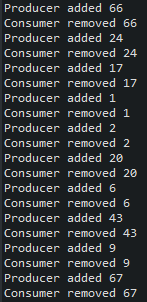
\includegraphics[height=2.5in, width = 1.5in]{pcsem1.png}\\
\end{center}\\

\begin{center}
2. Random example 2\\
\vspace{5mm}

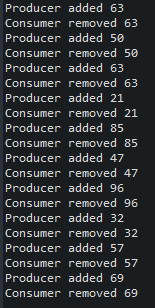
\includegraphics[height=2.5in, width = 1.5in]{pcsem2.png}\\
\end{center}\\

\begin{center}
\newpage
3. Random example 3\\
\vspace{10mm}

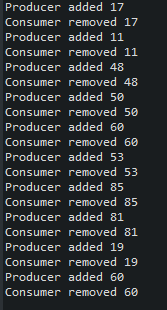
\includegraphics[height=2.5in, width = 1.5in]{pcsem3.png}\\
\end{center}\\

\section*{Solution Producer-Consumer with Monitors}\\
We use the synchronized keyword in order that 2 threads can't join the block at the same time. When the queue is empty the consumer waits, when the queue is full the producer waits. When a number is added to the queue the producer notifies, when a number is consumed from the queue the consumer notifies.
\begin{lstlisting}
//----------------------------PCQ.java----------------------------

import java.util.LinkedList;
import java.util.Queue;
import java.util.Random;

public class PCQ {
	int queueCapacity = 5;
	Random rand = new Random();
	int i;
	Queue<Integer> queue;
	PCQ(){
		queue = new LinkedList<>();
	}
	public void prod() throws InterruptedException
	{
		for(int it = 0 ; it < 10 ; it++)
		{
			synchronized(this)
			{
				while(queue.size() == queueCapacity)
					wait();
				i = rand.nextInt(100);
				System.out.println("Producer added " + i);
				queue.add(i);
				notify();
				Thread.sleep(500);
			}
		}
	}
	
	public void cons() throws InterruptedException
	{
		for(int it = 0; it < 10; it++)
		{
			synchronized (this)
			{
				while(queue.isEmpty())
					wait();
				System.out.println("Consumer removed " + queue.remove());
				notify();
				Thread.sleep(2000);
			}
		}
	}
}

\end{lstlisting}
\newpage
\section*{Experiments and results for producer-consumer with monitors}
\\\\\\
\begin{center}
Both the producer and consumer will do 10 steps. The queue capacity I've used for this example is 5.\\
1. Random example 1\\
\vspace{10mm}

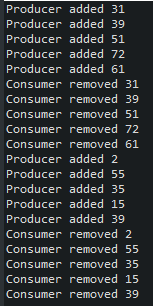
\includegraphics[height=2.5in, width = 1.5in]{pcmon1.png}\\
\end{center}\\
\begin{center}
2. Random example 2\\
\vspace{10mm}

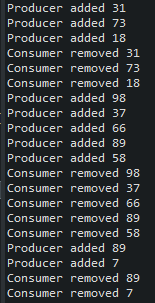
\includegraphics[height=2.5in, width = 1.5in]{pcmon2.png}\\
\end{center}\\

\begin{center}
\newpage
3. Random example 3\\
\vspace{10mm}

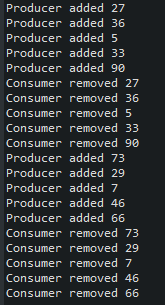
\includegraphics[height=2.5in, width = 1.5in]{pcmon3.png}\\
\end{center}\\

\newpage

\section*{Solution Producer-Consumer with Locks}\\
We use lock.lock() and lock.unlock() methods to keep the block available only to one thread. We also use two conditions which are the replacement for monitor methods( wait, await, etc). The conditions are for the cases when queue is full and empty.
\begin{lstlisting}
//----------------------------PCQ.java----------------------------

import java.util.LinkedList;
import java.util.Queue;
import java.util.Random;
import java.util.concurrent.locks.Condition;
import java.util.concurrent.locks.Lock;
import java.util.concurrent.locks.ReentrantLock;

public class PCQ {
	int queueCapacity = 5;
	Random rand = new Random();
	int i;
	Queue<Integer> queue;
	Lock lock;
	Condition notFull;
	Condition notEmpty;
	PCQ(){
		queue = new LinkedList<>();
		lock =  new ReentrantLock();
		notFull = lock.newCondition();
		notEmpty = lock.newCondition();
	}
	public void prod() throws InterruptedException
	{
		for(int it = 0 ; it < 10 ; it++)
		{
			lock.lock();
			try {
				while(queue.size() == queueCapacity)
					notEmpty.await();
				i = rand.nextInt(100);
				System.out.println("Producer added " + i);
				queue.add(i);
				Thread.sleep(500);
				notFull.signalAll();
			}
			finally {
				lock.unlock();
			}
		}
	}
	
	public void cons() throws InterruptedException
	{
		for(int it = 0; it < 10; it++)
		{
			lock.lock();
			try {
				while(queue.isEmpty())
					notFull.await();
				System.out.println("Consumer removed " + queue.remove());
				Thread.sleep(2000);
				notEmpty.signalAll();
			}
			finally {
				lock.unlock();
			}
		}
	}
}


\end{lstlisting}
\newpage
\section*{Experiments and results for producer-consumer with locks}
\\\\\\
\begin{center}
Both the producer and consumer will do 10 steps. The queue capacity I've used for this example is 5.\\
1. Random example 1\\
\vspace{10mm}

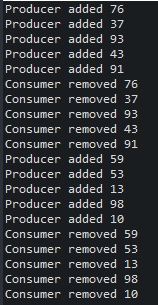
\includegraphics[height=2.5in, width = 1.5in]{pclock1.png}\\
\end{center}\\
\begin{center}
2. Random example 2\\
\vspace{10mm}

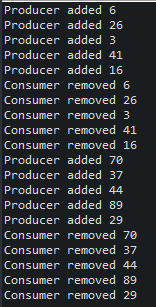
\includegraphics[height=2.5in, width = 1.5in]{pclock2.png}\\
\end{center}\\

\begin{center}
\newpage
3. Random example 3\\
\vspace{10mm}

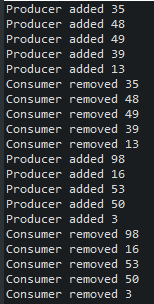
\includegraphics[height=2.5in, width = 1.5in]{pclock3.png}\\
\end{center}\\


\section*{Conclusions Producer-Consumer problem}
\vspace{10 mm}
The main problem we need to avoid is the deadlock. That's why we need to check everytime if the queue is full or empty. All the synchronization methods(locks, monitors, semaphores) have the same result, and the same efficiency. The reason we've implemented all is just for learning. I've started from the code presented at the laboratory and implemented the other synchronization methods on the same example.

\newpage
\section*{Common code for all the Dinning Philosophers implementations}\\
\begin{lstlisting}
//----------------------------Philosopher.java----------------------------

public class Philosopher extends Thread {
	public int philosopherId;
    private Fork leftFork;
    private Fork rightFork;
    public boolean stop = false;
    int hasEat = 0;

    public Philosopher(int id, Fork leftFork , Fork rightFork ) {
      this.philosopherId = id;
      this.leftFork = leftFork;
      this.rightFork = rightFork;
    }

    @Override
    public void run() {

      try {
        while (!stop) {
          think();
          if (leftFork.pickUp("Philosopher-" + philosopherId, "left")) {
            if (rightFork.pickUp("Philosopher-" + philosopherId, "right")) {
              eat();
              rightFork.putDown("Philosopher-" + philosopherId, "right");
            }
            leftFork.putDown("Philosopher-" + philosopherId, "left");
          }
        }
      } catch (Exception e) {
        e.printStackTrace();
      }
    }

    private void think() throws InterruptedException {
      System.out.println("Philosopher-" + philosopherId + " is thinking");
      Thread.sleep(1000);
    }

    private void eat() throws InterruptedException {
      System.out.println("Philosopher-" + philosopherId + " is eating");
      hasEat++;
      Thread.sleep(1000);
    }
}

\end{lstlisting}
\begin{lstlisting}
//----------------------------Main.java----------------------------


public class Main {

	public static void main(String[] args) throws InterruptedException {
		int philosophersNumber = 5;

	    Philosopher[] philosophers = null;

	      philosophers = new Philosopher[philosophersNumber];
	      Fork[] forks = new Fork[philosophersNumber];
	      
	      for (int i = 0; i < philosophersNumber; i++) {
	    	  forks[i] = new Fork(i);
	      }

	      for (int i = 0; i < philosophersNumber; i++) {
	        philosophers[i] = new Philosopher(i, forks[i], forks[(i + 1) % philosophersNumber]);
	        philosophers[i].start();
	      }
	      Thread.sleep(10000);
	      for (Philosopher philosopher : philosophers) { 
	        philosopher.stop = true;
	        philosopher.join();
	      }
	      for (Philosopher philosopher2 : philosophers)
	          System.out.println("Philosopher-" + philosopher2.philosopherId + " has eat " + philosopher2.hasEat);

	}
}


\end{lstlisting}

\section*{Solution Producer-Consumer with Semaphores}\\
The solution I've implemented uses one semaphore for each fork. This semaphore locks fork when it's picked up and releases it when it's put down. This way two philosophers can't pick the same fork at the same time.

\begin{lstlisting}
//----------------------------Fork.java----------------------------

import java.util.concurrent.Semaphore;
import java.util.concurrent.locks.Lock;
import java.util.concurrent.locks.ReentrantLock;

public class Fork {
	Semaphore sem = new Semaphore(1);
    private final int ForkId;

    public Fork(int id) {
      this.ForkId = id;
    }

    public boolean pickUp(String name, String where) throws InterruptedException {
      if (sem.tryAcquire()) {
        System.out.println(name + " picked up " + where + " fork-" + ForkId);
        return true;
      }
      return false;
    }

    public void putDown(String name, String where) {
    	sem.release();
      System.out.println(name + " put down " + where + " fork-" + ForkId);
    }
}


\end{lstlisting}

\vspace{5 mm}\\
\section*{Experiments and results for Dinning Philosophers with semaphores}
\\\\\\
\begin{center}
The code will run for 5 seconds and will have 2 philosophers. More experiments with bigger number of philosophers/time will be found in the Experiments and data results folder\\
\newpage{}
1. Random example 1\\
\vspace{5mm}
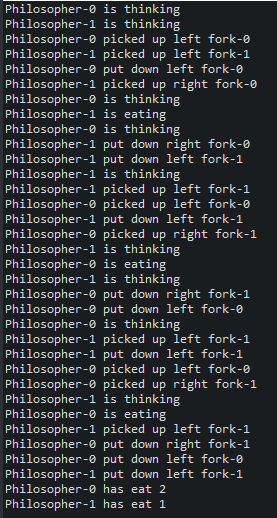
\includegraphics[height=3.2in, width = 2.5in]{philosem1.png}\\
\end{center}\\

\begin{center}
2. Random example 2\\
\vspace{5mm}

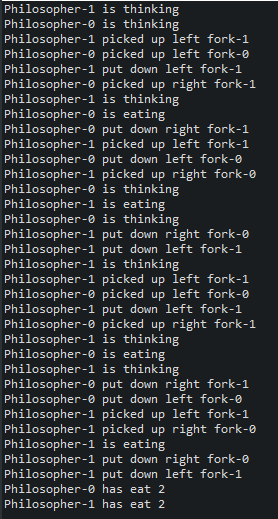
\includegraphics[height=3.2in, width = 2.5in]{philosem2.png}\\
\end{center}\\

\begin{center}
\newpage
3. Random example 3\\
\vspace{10mm}

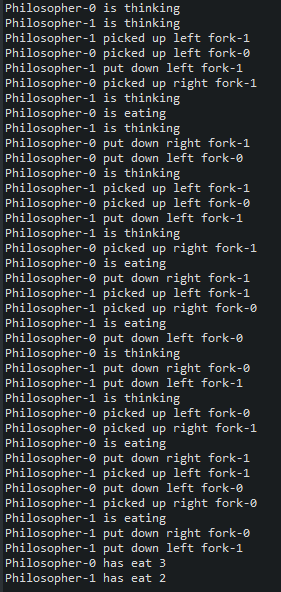
\includegraphics[height=3.2in, width = 2.5in]{philosem3.png}\\
\end{center}\\

\section*{Solution Dining Philosophers with Monitors}\\
We use the synchronized keyword in order that 2 threads can't join the block at the same time. So only one philospoher can pick the fork
\begin{lstlisting}
//----------------------------Fork.java----------------------------

public class Fork {
    private final int ForkId;
    static boolean state = false;

    public Fork(int id) {
      this.ForkId = id;
    }

    public synchronized boolean pickUp(String name, String where) throws InterruptedException {
      if (state == false) {
        System.out.println(name + " picked up " + where + " fork-" + ForkId);
        state = true;
        return true;
      }
      return false;
    }

    public synchronized void putDown(String name, String where) {
      System.out.println(name + " put down " + where + " fork-" + ForkId);
      state = false;
    }
}


\end{lstlisting}
\section*{Experiments and results for Dining Philosophers with monitors}
\\\\\\
\begin{center}
The code will run for 5 seconds and will have 2 philosophers. More experiments with bigger number of philosophers/time will be found in the Experiments and data results folder\\
1. Random example 1\\
\vspace{10mm}

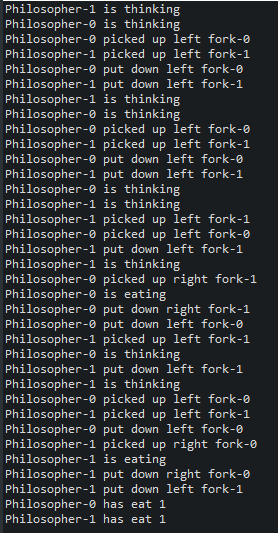
\includegraphics[height=3.2in, width = 2.5in]{philomon1.png}\\
\end{center}\\
\begin{center}
2. Random example 2\\
\vspace{10mm}

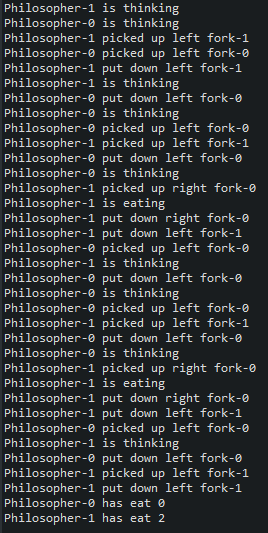
\includegraphics[height=3.2in, width = 2.5in]{philomon2.png}\\
\end{center}\\

\begin{center}
3. Random example 3\\
\vspace{10mm}

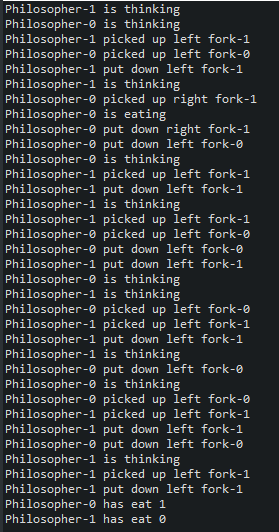
\includegraphics[height=3.2in, width = 2.5in]{philomon3.png}\\
\end{center}\\

\newpage

\section*{Solution Dining Philosophers with Locks}\\
We use lock() method when the fork is picked up and we release it when it's put down.
\begin{lstlisting}
//----------------------------Fork.java----------------------------

import java.util.concurrent.locks.Lock;
import java.util.concurrent.locks.ReentrantLock;

public class Fork {
    Lock lock = new ReentrantLock();
    private final int ForkId;

    public Fork(int id) {
      this.ForkId = id;
    }

    public boolean pickUp(String name, String where) throws InterruptedException {
      if (lock.tryLock()) {
        System.out.println(name + " picked up " + where + " fork-" + ForkId);
        return true;
      }
      return false;
    }

    public void putDown(String name, String where) {
    	lock.unlock();
      System.out.println(name + " put down " + where + " fork-" + ForkId);
    }
}

\end{lstlisting}
\section*{Experiments and results for producer-consumer with locks}
\\\\\\
\begin{center}
Both the producer and consumer will do 10 steps. The queue capacity I've used for this example is 5.\\
1. Random example 1\\
\vspace{10mm}

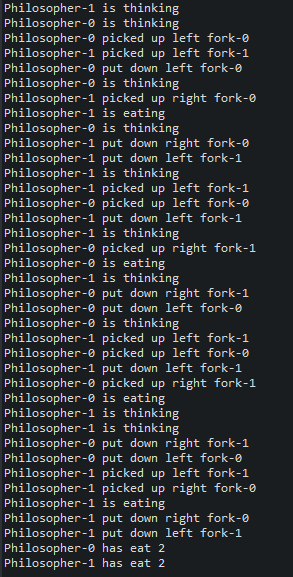
\includegraphics[height=3.2in, width = 2.5in]{philolock1.png}\\
\end{center}\\
\begin{center}
2. Random example 2\\
\vspace{10mm}

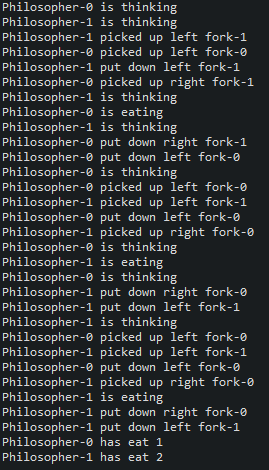
\includegraphics[height=3.2in, width = 2.5in]{philolock2.png}\\
\end{center}\\

\begin{center}
3. Random example 3\\
\vspace{10mm}

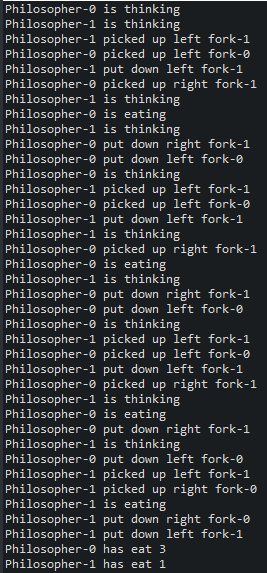
\includegraphics[height=3.2in, width = 2.5in]{philolock3.png}\\
\end{center}\\


\section*{Conclusions Dining Philosophers problem}
\vspace{10 mm}
The main problem we need to avoid is the deadlock. Each fork has a synchronization method( doesn't matter if it's a lock/monitor or semaphore because all of them are doing the same thing ). Each fork can be accesed only by one thread at a moment of time, this way two philosophers can't pick the same fork. I've learnt more about deadlocks and concurrent programming synchronization methods

\newpage
\section*{References}
https://en.wikipedia.org/wiki/Dining_philosophers_problem
\\
https://docs.oracle.com/javase/7/docs/api/java/util/concurrent/locks/Condition.html
\\

\end{document}